\section{First Exercise}
The matrix
\begin{singlespace} 
\begin{equation}
    \begin{pmatrix}
        1 & 0 & 0 & 0 & 0 & 0 & 0 & 0\\
        0 & 1 & 0 & 0 & 0 & 0 & 0 & 0\\
        0 & 0 & 1 & 0 & 0 & 0 & 0 & 0\\
        0 & 0 & 0 & 1 & 0 & 0 & 0 & 0\\
        0 & 0 & 0 & 0 & a & 0 & 0 & c\\
        0 & 0 & 0 & 0 & 0 & 1 & 0 & 0\\
        0 & 0 & 0 & 0 & 0 & 0 & 1 & 0\\
        0 & 0 & 0 & 0 & b & 0 & 0 & d\\
    \end{pmatrix}
\end{equation}
\end{singlespace}
acts non-trivially on the states $\ket{100}$ and $\ket{111}$. Thus we can write a Gray code
\begin{singlespace}
\begin{equation}
    \begin{matrix}
        A & B & C\\
        1 & 0 & 0\\
        1 & 1 & 0\\
        1 & 1 & 1\\
    \end{matrix}
\end{equation}
\end{singlespace}
That is, we need a three-qubit operation switching the second qubit before applying the unitary operator $U^T$ where 
\begin{singlespace}
\begin{equation}
    U = \begin{pmatrix}
        a & b\\
        c & d\\
    \end{pmatrix},
\end{equation}
\end{singlespace}
which would look like
\begin{figure}[H]
    \centering
    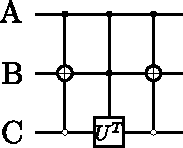
\includegraphics{threeQBcircuit.pdf}
\end{figure}
However, we want to show this with only single-qubit operations and two-qubit operations. This is shown in the next page. It is very wide so can be a bit hard to see. The red parts are the CCNOT gates while the blue part is the double controlled $U^T$ part, where $V$ is a unitary operator such that $V^2 = U^T$

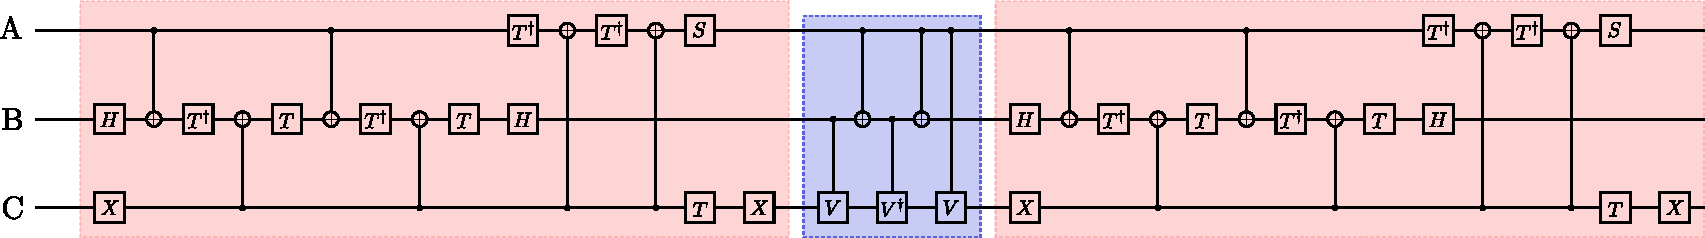
\includepdf[fitpaper=true]{figures/circuit.pdf}